\section{Biopsychism and Biological Naturalism}

ECC aligns closely with both biopsychist perspectives and biological naturalism, though it offers distinct contributions to each framework through its emphasis on energetic coherence and cellular organization. Like biopsychism, ECC locates consciousness at the cellular level, suggesting that conscious experience emerges from the fundamental properties of living systems \cite{edwards2005consciousness, shapiro2007bacteria}. However, ECC specifies that this emergence requires particular forms of energetic coherence and organization that are characteristic of biological systems, especially neural and glial networks.

From biological naturalism, ECC inherits the view that consciousness is irreducibly grounded in biological processes \cite{searle2017biological}. However, while traditional biological naturalism focuses primarily on neural systems, ECC expands this view to encompass broader cellular and energetic dynamics. This expansion allows ECC to bridge the gap between simpler cellular awareness and complex conscious experience through its framework of energetic coherence \cite{van2006principles}.

The cellular foundations of consciousness in ECC parallel biopsychist insights, but with crucial distinctions. While both approaches recognize consciousness at the cellular level \cite{lyon2015cognitive}, ECC emphasizes that these cellular processes must achieve specific forms of energetic coherence to support consciousness. This requirement distinguishes ECC from broader forms of biopsychism that might attribute consciousness to all cellular activity without qualification \cite{margulis2000life}.

The energetic organization principles of ECC provide a mechanistic framework for understanding how biological systems generate conscious experience. While biological naturalism emphasizes the biological basis of consciousness \cite{searle1992rediscovery}, ECC specifies that the critical biological features are those that enable coherent energy flows and stable feedback systems. This focus on energetic organization provides concrete mechanisms for understanding how biological systems generate conscious experience, moving beyond both general biopsychist claims and traditional biological naturalist approaches \cite{thompson2010mind}.

ECC suggests that complex consciousness emerges from the integration of cellular-level coherence into broader, stable fields through mechanisms like astrocytic syncytia and transcriptomic profiles. This multi-level integration explains how simple cellular awareness can scale to complex conscious experience while maintaining the biological grounding emphasized by both biopsychism and biological naturalism \cite{godfrey2016other}.

Within an evolutionary context, ECC's framework provides an account that aligns with both perspectives while offering additional specificity \cite{varela1997patterns}. It suggests that consciousness evolved as biological systems developed increasingly sophisticated mechanisms for maintaining energetic coherence, beginning with cellular processes and culminating in the complex neural systems of modern organisms \cite{deacon2011incomplete}.

Through this synthesis, ECC offers a framework that preserves the key insights of both biopsychism and biological naturalism while providing a more specific mechanism - energetic coherence - for understanding how biological systems generate conscious experience. This approach suggests that consciousness is neither a universal property of all biological systems nor limited to neural activity alone, but rather emerges from specific forms of energetically coherent biological organization \cite{clark2010supersizing}.

\begin{figure}[h]
    \centering
    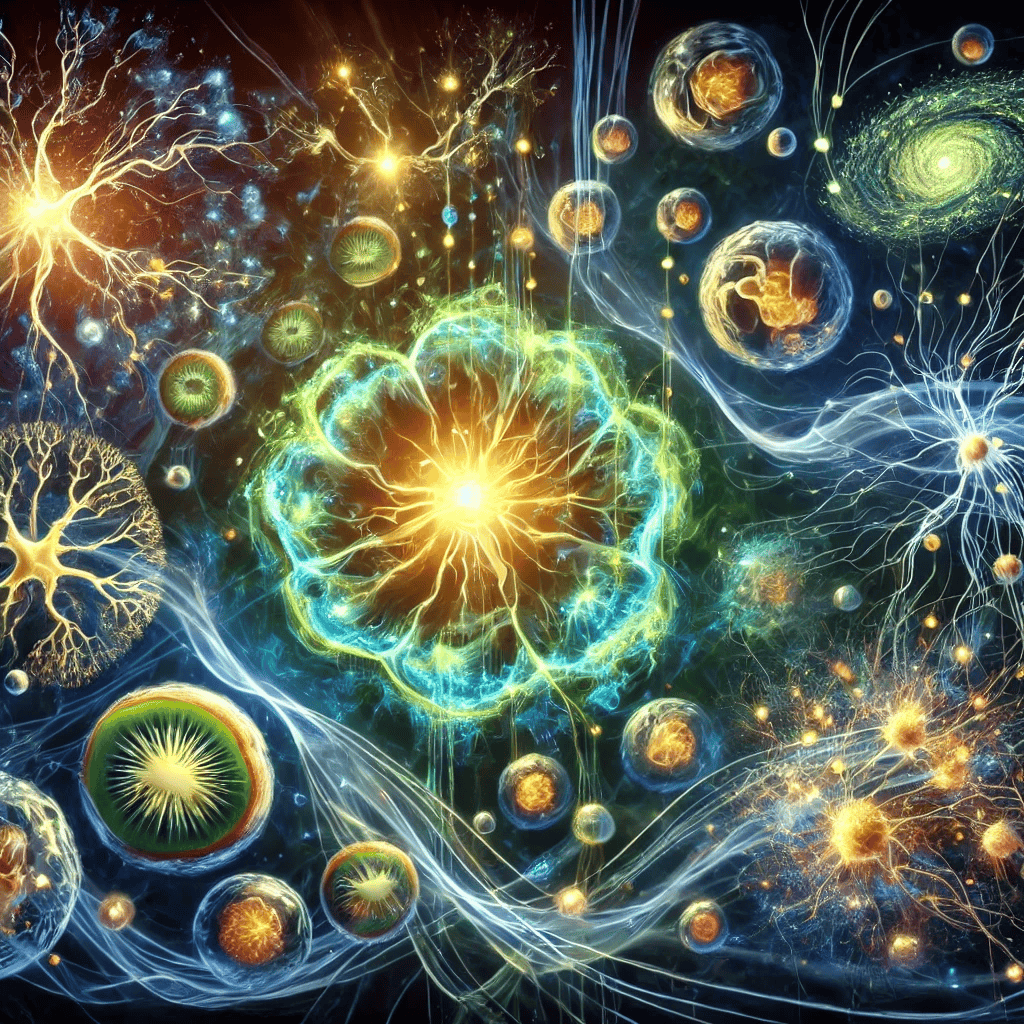
\includegraphics[width=0.8\textwidth]{conscious_cells.png}

    \caption{Biopsychism - cells are conscious}
\end{figure}

The relationship between cellular organization and conscious experience takes on particular significance in ECC's framework. Through specific patterns of energetic coherence, cellular networks achieve forms of integration that transcend simple aggregation \cite{lyon2015cognitive}. These patterns emerge through the interplay of membrane dynamics, ion gradients, and bioelectric fields that characterize living systems. Unlike traditional biological naturalism, which might treat these features as mere implementation details \cite{searle2017biological}, ECC positions them as fundamental to the generation of conscious states.

The role of transcriptomic profiles in shaping conscious capacity represents another crucial advance in ECC's synthesis \cite{Tasic2018,Hawrylycz2012}. Different cell populations maintain distinct molecular configurations that enable particular forms of energetic coherence \cite{shapiro2007bacteria}. This molecular diversity creates what ECC terms a rich alphabet of possible conscious states, explaining both how consciousness can maintain stability and how it can support sophisticated information processing. This perspective bridges the seeming gap between cellular-level awareness and complex conscious experience \cite{van2006principles}.

ECC's treatment of astrocytic networks provides a concrete example of how its framework extends beyond both biopsychism and biological naturalism. These networks create continuous domains of coordinated activity through gap junctions and calcium waves, establishing coherent fields that span multiple cellular populations \cite{edwards2005consciousness}. This mechanism demonstrates how consciousness can emerge at scales beyond individual cells while remaining grounded in cellular processes \cite{thompson2010mind}.

The framework particularly illuminates the relationship between metabolism and consciousness. Where traditional approaches might treat energy management as merely supportive of conscious processing \cite{searle1992rediscovery}, ECC suggests that specific patterns of energetic organization are constitutive of consciousness itself. This helps explain why consciousness requires such sophisticated cellular machinery while avoiding claims that all metabolic processes generate consciousness \cite{margulis2000life}.

Through careful attention to boundary conditions, ECC provides new insight into the limits of conscious experience. The framework suggests that consciousness emerges only when cellular systems achieve sufficient coherence to maintain stable yet dynamic energy states \cite{varela1997patterns}. This explains both why consciousness appears limited to certain biological systems and how it can support such remarkable flexibility within those constraints \cite{godfrey2016other}.

The interaction between cellular and network-level processes takes on new significance through ECC's lens. Rather than treating these as separate levels of organization, the framework shows how they represent different scales of coherent energy dynamics \cite{lyon2015cognitive}. This multi-scale integration helps explain how consciousness can maintain both local specificity and global unity, a feature that has challenged both biopsychist and biological naturalist accounts \cite{clark2010supersizing}.

This theoretical synthesis has important practical implications for understanding disorders of consciousness and potential therapeutic interventions. By identifying specific mechanisms through which conscious states emerge from cellular processes \cite{deacon2011incomplete}, ECC suggests new approaches to treating conditions that affect consciousness. This demonstrates how the framework moves beyond philosophical positions to generate concrete insights for medical applications \cite{thompson2010mind}.

The synthesis of biopsychist and biological naturalist perspectives in ECC ultimately points toward a fundamental insight: consciousness cannot be reduced to computational processes alone, regardless of their complexity \cite{thompson2010mind}. This departure from computational theories of mind emerges naturally from ECC's emphasis on physical dynamics and energetic coherence in biological systems \cite{searle2017biological}.

The energetic requirements for consciousness, as revealed through ECC's analysis of cellular and systemic organization, demonstrate why computation alone proves insufficient for generating conscious experience \cite{varela1997patterns}. While computational processes can simulate or model aspects of consciousness, they cannot replicate the fundamental coherence that emerges from continuous, physically-grounded energy dynamics. This insight helps resolve longstanding debates about the possibility of machine consciousness while explaining why biological systems remain uniquely capable of supporting conscious experience \cite{lyon2015cognitive}.

The framework's emphasis on physical implementation extends beyond traditional arguments about substrate dependence \cite{edwards2005consciousness,polger2016multiple}. Rather than simply claiming that consciousness requires particular physical structures, ECC demonstrates how specific patterns of energetic coherence, maintained through sophisticated biological machinery, create the conditions necessary for conscious experience \cite{shapiro2007bacteria}. These patterns cannot be reduced to abstract information processing but require continuous, physically-grounded processes that integrate multiple scales of biological organization \cite{van2006principles}.

This non-computational nature of consciousness becomes particularly evident when examining how biological systems achieve coherent integration across different scales \cite{margulis2000life}. Unlike digital computers that maintain sharp boundaries between processing elements, conscious systems operate through continuous fields of influence that span multiple levels of organization. The resulting integration cannot be achieved through discrete computational steps but requires physical processes that maintain coherence through direct energetic interaction \cite{godfrey2016other}.